\documentclass{article}
\usepackage{setspace,tikz}
\usepackage[text={6.5in,8.5in},centering]{geometry}
\geometry{verbose,a4paper,tmargin=2.4cm,bmargin=2.4cm,lmargin=2.4cm,rmargin=2.4cm}
\usepackage{graphicx,amsmath,cases,multirow,appendix,graphicx,xcolor}

\setlength\parindent{0pt}

\newcommand{\note}[1]{\colorbox{gray!30}{#1}}
\newcommand{\ind}{\-\hspace{1cm}}
\newcommand*\circled[1]{\tikz[baseline=(char.base)]{
            \node[shape=circle,draw,inner sep=2pt] (char) {#1};}}

\begin{document}

\noindent\makebox[\textwidth][c]{\Large\bfseries Lecture 10 -- Two-species competition}

\rule[0.5ex]{\linewidth}{1pt}
\textbf{Today:} Graphical analysis of two-species competition.\\
\textbf{Next:} 2-D stability analysis\\
\textbf{Concepts for the road ahead:}\\
\ind Coexistence, Invasibility, Priority effects, Alternative Stable States\\
\ind Phase diagrams \& Zero Net Growth Isoclines (ZNGI's) \\
\rule[0.5ex]{\linewidth}{1pt}

\textbf{Two-species competition} \ind \note{Motivate with Crombie (1946) flour beetle experiments. 2 slides.}\\
Extend 1 sp. logistic to 2 spp.
\begin{align*}
	\frac{dN_1}{dt}=r_1 N_1 \left (1-\frac{N_1}{K_1} - \alpha_{12}\frac{N_2}{K_1}\right) \quad \quad
	\frac{dN_2}{dt}=r_2 N_2 \left (1-\frac{N_2}{K_2} - \alpha_{21}\frac{N_1}{K_2}\right)
\end{align*}
Or in slightly different general form:
\begin{equation*}
	\frac{dN_i}{dt}=r_i N_i \left (1-\frac{N_i}{K_i} - \alpha_{ij}\frac{N_j}{K_i}\right) \quad \mbox{ for } i \neq j.
\end{equation*}
Contrast \emph{intra}-specific density-dependence (self-limitation) vs. \emph{inter}-specific competition

$\alpha_{ij}$ - effect of 1 average $j$ individual on 1 average $i$ individual relative to effect that $i$ has on self.\\
\ind \ind  = per capita effect\\
\ind \ind 'How much of $K_i$ does each $j$ individual use?'\\
\ind \ind \ind e.g., if 10 $j$ individuals consume equivalent to 1 $i$ individual, then $\alpha_{ij}=\tfrac{1}{10}$.\\

This is a model of \textbf{exploitation} with \emph{implicit} resources.\\
\textbf{Implicit} - Resource dynamics are \emph{not} modeled\\
\ind \ind - Phenomenological model depiction of resources\\
\ind \ind - e.g., $K$ - 'carrying capacity'\\
That is:
\begin{equation*}
	\frac{dN_i}{dt}=f_i(N_i,N_j)
\end{equation*}
\begin{center}
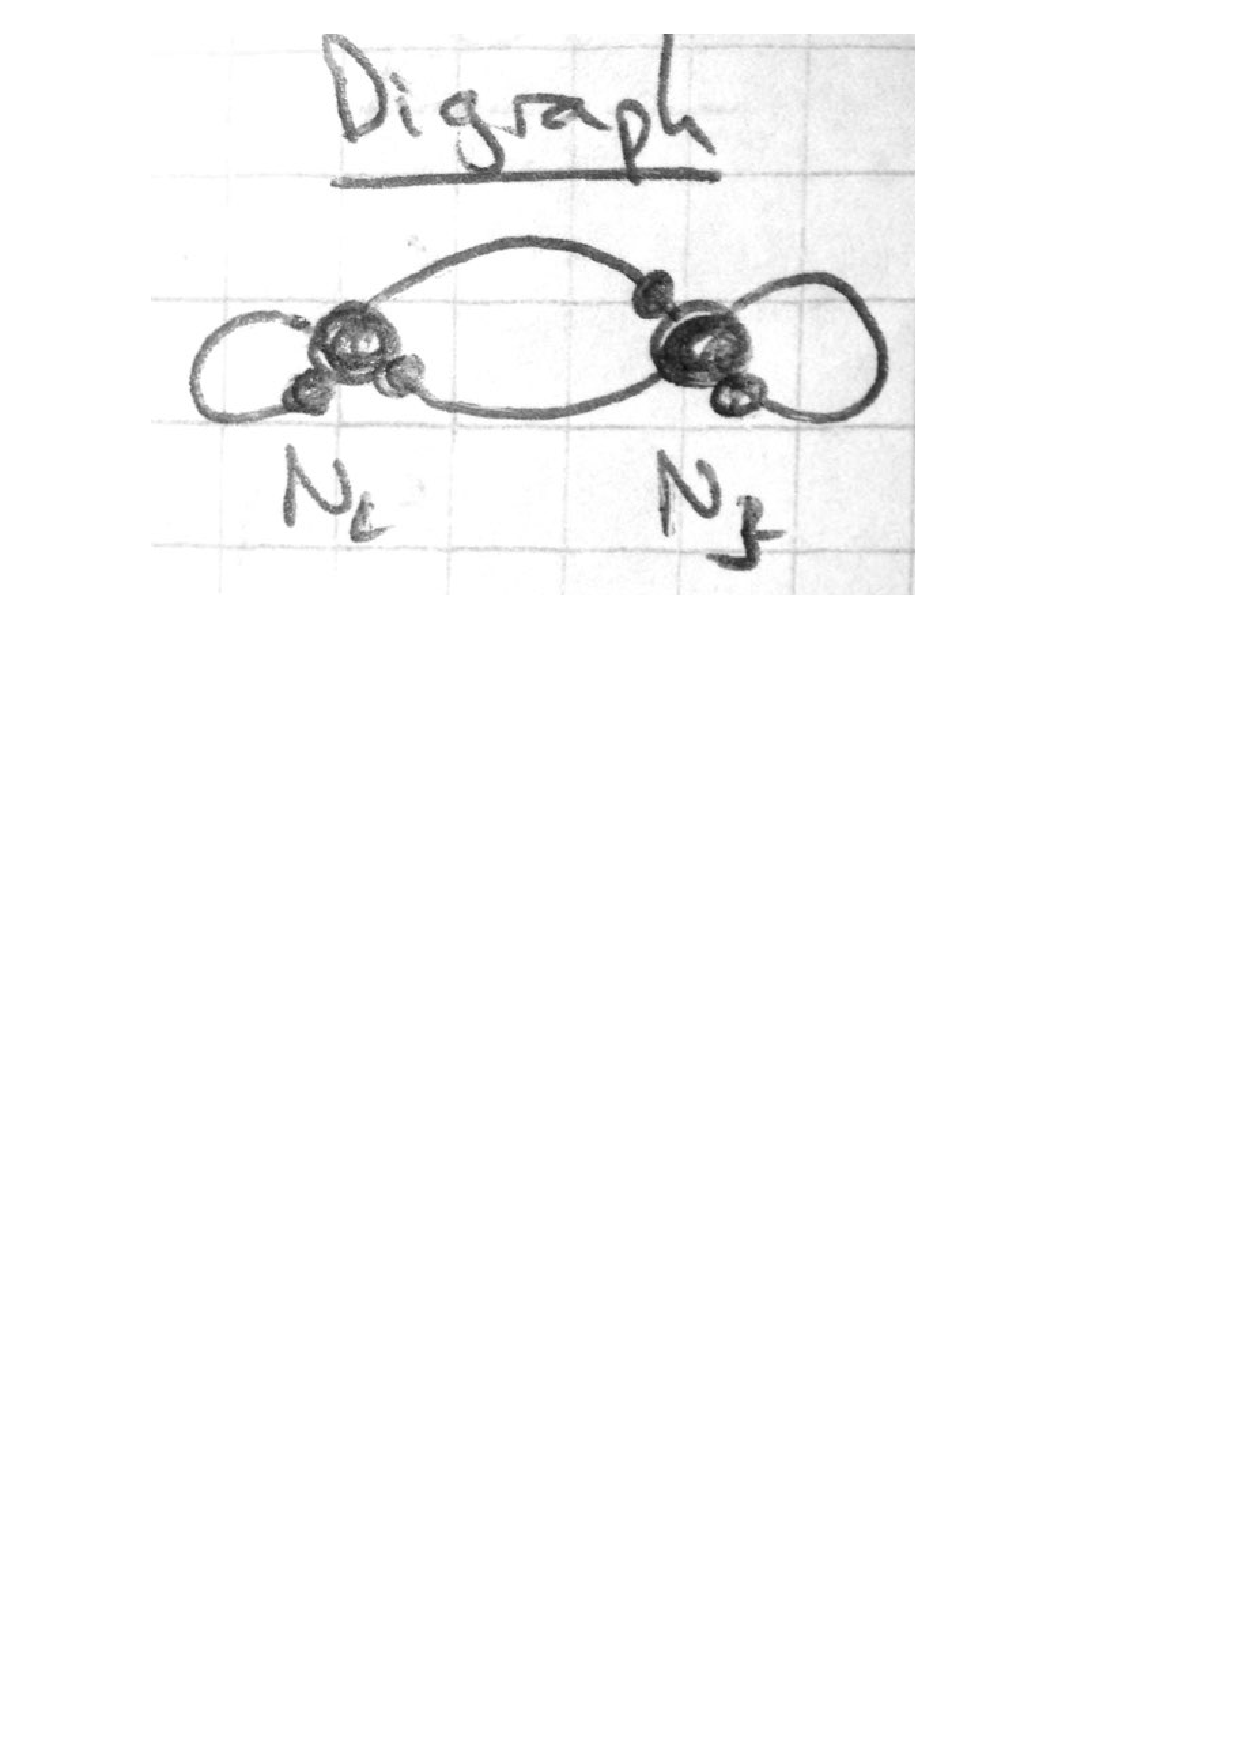
\includegraphics[width=2cm]{figs/Digraph_implicit.pdf}
\end{center}

\textbf{Explicit} - Resource dynamics \emph{are} modeled\\
\ind \ind e.g. Consumer-resource models (\note{next class})
\begin{align*}
	\frac{dN_i}{dt}=f_i(N_i,R) \quad \quad 
	\frac{dR}{dt}=f_R(N_i,N_j,R)
\end{align*}
\begin{center}
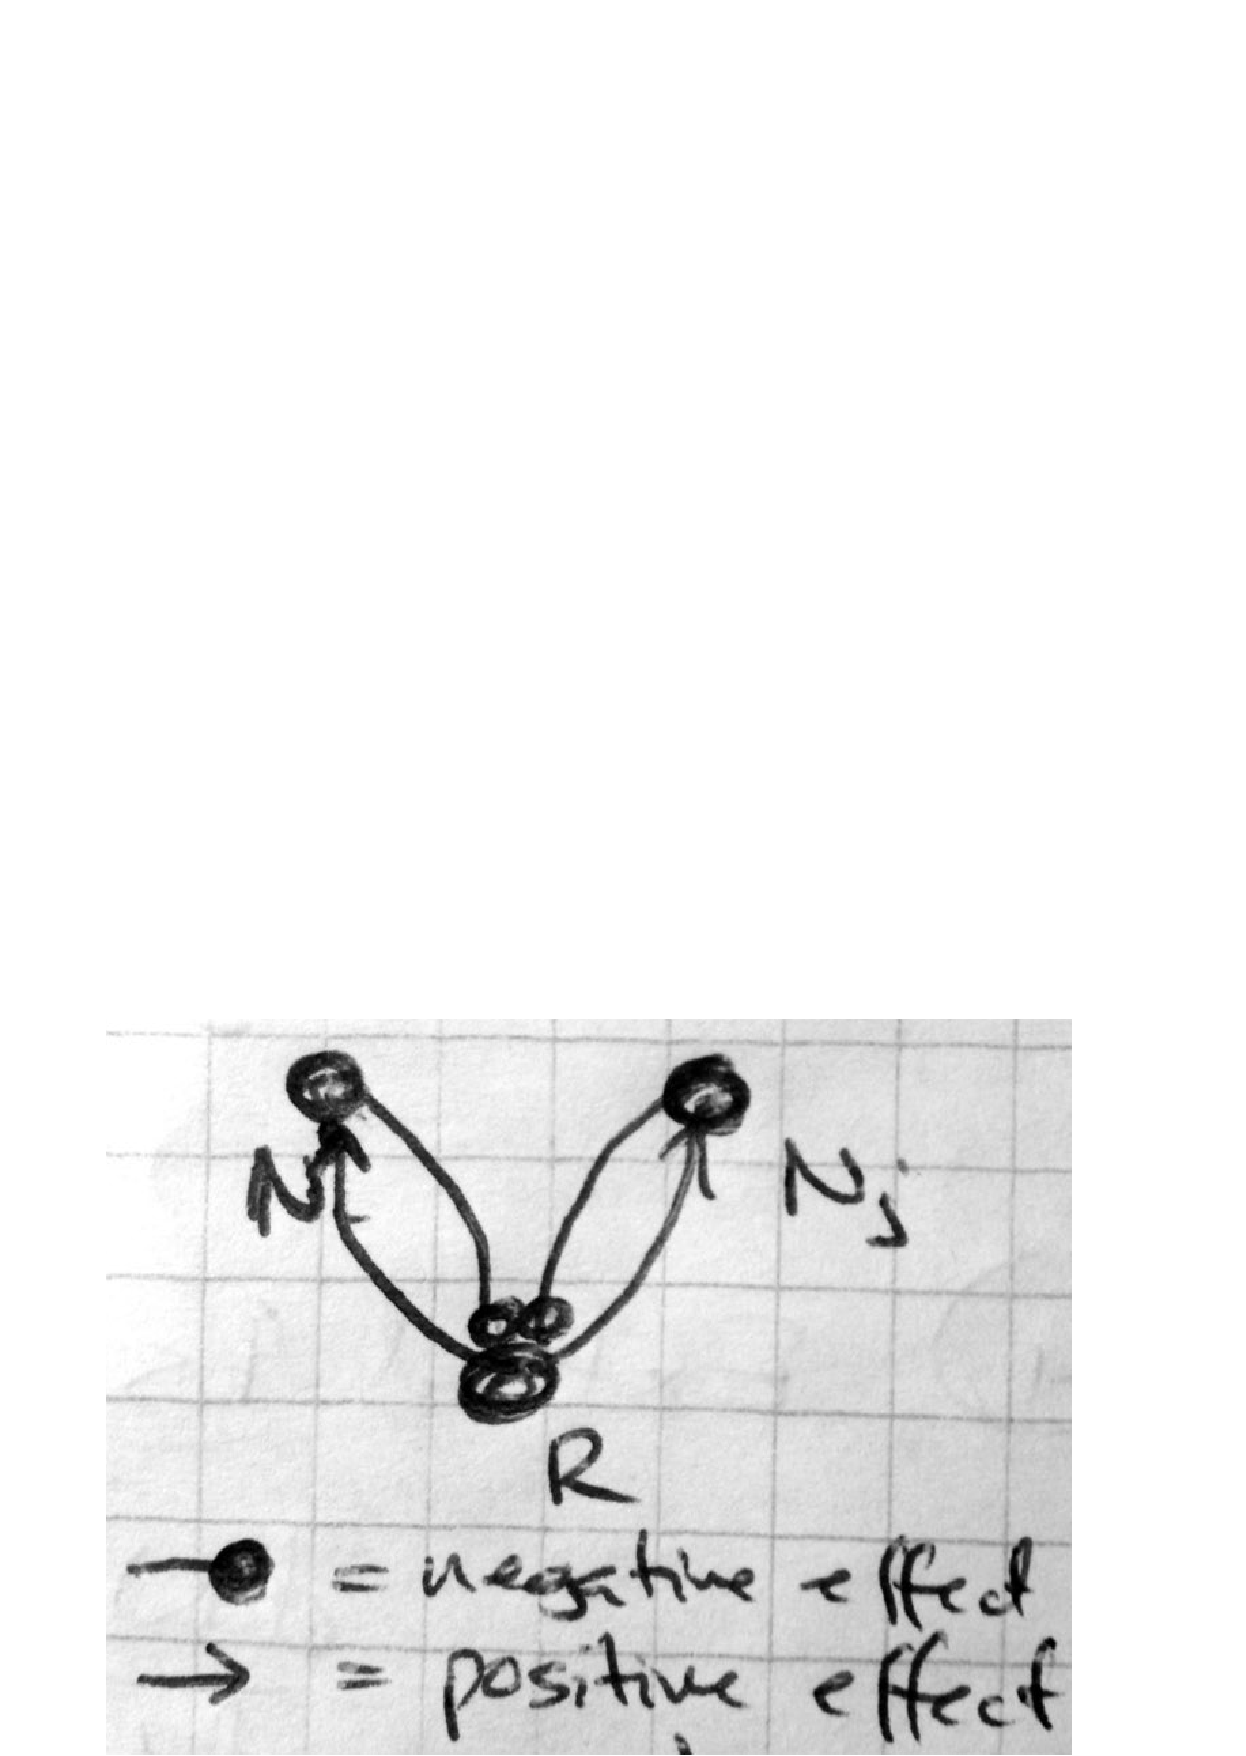
\includegraphics[width=2cm]{figs/Digraph_explicit.pdf}
\end{center}

\textbf{Exploitation} - Indirect negative interaction through joint use of shared \emph{limiting} resource(s).

\textbf{Interference} - Direct negative interaction preventing use of resource(s).

\rule[0.5ex]{\linewidth}{1pt}

\textbf{Today's Q:} \\ 
\ind When can two species coexist on the same shared resource(s)?\\
\ind When can Sp. 1 invade a community consisting of Sp. 2?\\
\ind \ind $\Rightarrow$ How many equilibria are there?\\
\ind \ind $\Rightarrow$ Are equilibria stable or unstable?\\

\rule[0.5ex]{\linewidth}{1pt}
\pagebreak

\note{Hand out and work through quiz as group:}
(a)
\begin{equation*}
		\frac{dN_i}{dt}=r_i N_i \left (1-\frac{N_i}{K_i} - \alpha_{ij}\frac{N_j}{K_i}\right)
\end{equation*}
Qualitatively...
\begin{align*}
(N_i^*,N_j^*)& =
\begin{cases}
	0, & 0  \\
	N_i^* > 0, & 0  \\
	0, & N_j^* > 0\\
	N_i^* > 0, & N_j^* > 0
\end{cases}
\end{align*}

(b)\\
When $N_j=0$ $\Rightarrow$ reduces to 1 sp. logistic:
\begin{align*}
	\frac{dN_i}{dt} & =r_i N_i \left (1-\frac{N_i}{K_i} \right)\\
	N_i^*  & = K_i
\end{align*}

(c)\\
Replace $i$ for $j$, $\Rightarrow N_j^* = K_j$ in absence of $i$.\\

(d)\\
Want $N_i^* > 0$ \&  $N_j^* > 0$\\
A: Solve for one as function of the other:\\
\begin{align*}
	r_i N_i - \frac{r_i N_i N_i}{K_i} - \frac{ r_i \alpha_{ij} N_i N_j}{K_i} & =0\\
	r_i N_i K_i & = r_i N_i N_i + r_i \alpha_{ij} N_i N_j   \quad \quad \text{(move and  multiply by }K_i)\\
	K_i & = N_i + \alpha_{ij}N_j  \quad \quad (\text{divide by } r_i \text{  and } N_i)\\[1em]
	N_i^* & = K_i - \alpha_{ij} N_j  \quad \text{ and similarly }	N_j^* = K_j - \alpha_{ji} N_i
%	\\
%	[1em]
%	\text{ or, rearranging differently} \\
%	K_i - N_i^* & = \alpha_{ij} N_j\\
%	N_j & = \frac{K_i - N_i^*}{\alpha_{ij}} \quad \text{ and } N_i  = \frac{K_j - N_j^*}{\alpha_{ji}}
 \end{align*}
 
Note intuitive meaning of $\alpha_{ij}$!\\
Note also that we can't solve for one species without knowing the other.\\
\ind $\Rightarrow$ need to solve for $N_i^*$ and $N_j^*$ jointly.\\
\ind Plug solution of $N_j^*$ into solution for $N_i^*$ and vice versa.
\begin{align*}
	N_i^*  & = K_i - \alpha_{ij} N_j^* \\
				& = K_i - \alpha_{ij} \left ( K_j  - \alpha_{ji} N_i^* \right )\\
				& = K_i - \alpha_{ij} K_j + \alpha_{ij}\alpha_{ji} N_i^* \\
	N_i^* + \alpha_{ij} K_j - \alpha_{ij} \alpha_{ji} N_i^* & = K_i \\
	N_i^* - \alpha_{ij} \alpha_{ji} N_i^* & = K_i - \alpha_{ij} K_j \\
	N_i^* \left (1 - \alpha_{ij} \alpha_{ji} \right)  & = K_i - \alpha_{ij} K_j \\
	N_i^* & = \frac{ K_i - \alpha_{ij} K_j  } {1-\alpha_{ij} \alpha_{ji} }
\end{align*}

\rule[0.5ex]{\linewidth}{1pt}

\pagebreak
\textbf{Phase portraits/diagrams}\\
\note{R-code demonstration}\\
\ind \note{Work through ode-solver code}\\
\ind \note{Simulate coexistence over time}
\begin{center}
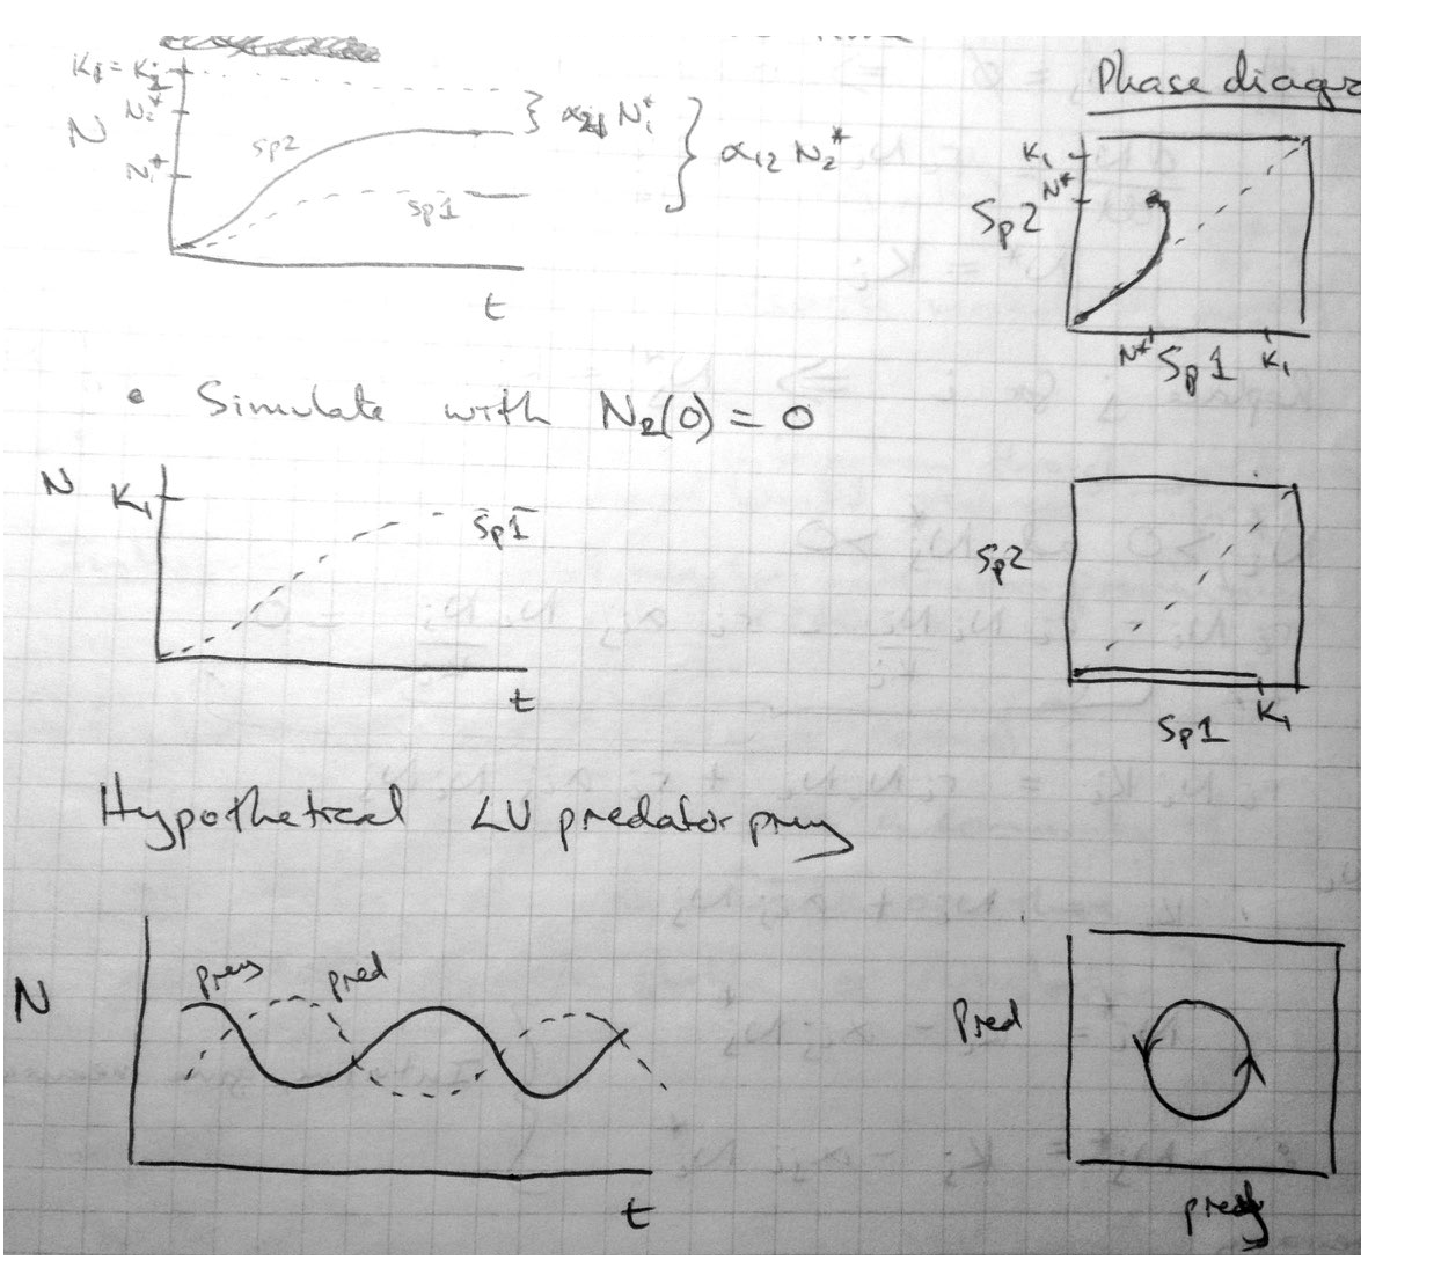
\includegraphics[width=15cm]{figs/PhasePortraits.pdf}
\end{center}

\rule[0.5ex]{\linewidth}{1pt}

Return to main questions:\\
\ind When can both spp. coexist?\\
\ind When can sp 1 out-compete sp 2?\\
\ind When can sp 1 invade sp 2?\\

\textbf{Naive simulations}\\
\ind \note{R-demonstration - Walk through first set of parameter values. ``Naive simulations''}\\
\ind \ind \note{Then show full table before showing results with R code for other parameters.}\\

\ind With $r_1 = r_2 = K_1 = K_2 = 1$ and $N_1(0) = N_2(0)=0.01$

\begin{table*}[h]
\centering
\begin{tabular}{cccc}
$\alpha_{21}$ & $\alpha_{12}$ & Outcome \\ 
\hline
0.5 & 0.7 & coexist & \\
1.5 & 0.5 & sp1 & \\
0.5 & 1.5 & sp2 & $N_1(0)=N_2(0)$\\
1.5 & 1.7 & sp2 & \\
\hline
1.5 & 1.7 & sp1 & $N_1(0)>N_2(0)$\\
 \hline
\end{tabular} 
\end{table*}
\ind \ind \ind \ind \ind \ind $\Rightarrow$ Priority effect\\
\ind \ind \ind \ind \ind \ind  $\Rightarrow$ Alternative stable states

\textbf{Graphical Analysis}\\
Earlier we showed that from $\frac{dN_i}{dt}=0$ that:
\begin{align*}
	N_i^* = & K_i - \alpha_{ij} N_j\\
	\Rightarrow N_j = & \frac{K_i-N_i^*}{\alpha_{ij}}\\
	\text{Thus isocline interesects x-axis at}\\
  N_j = & \frac{K_i-0}{\alpha_{ij}}=\frac{K_i}{\alpha_{ij}}
	\end{align*}

Same goes for 2nd species.
\begin{center}
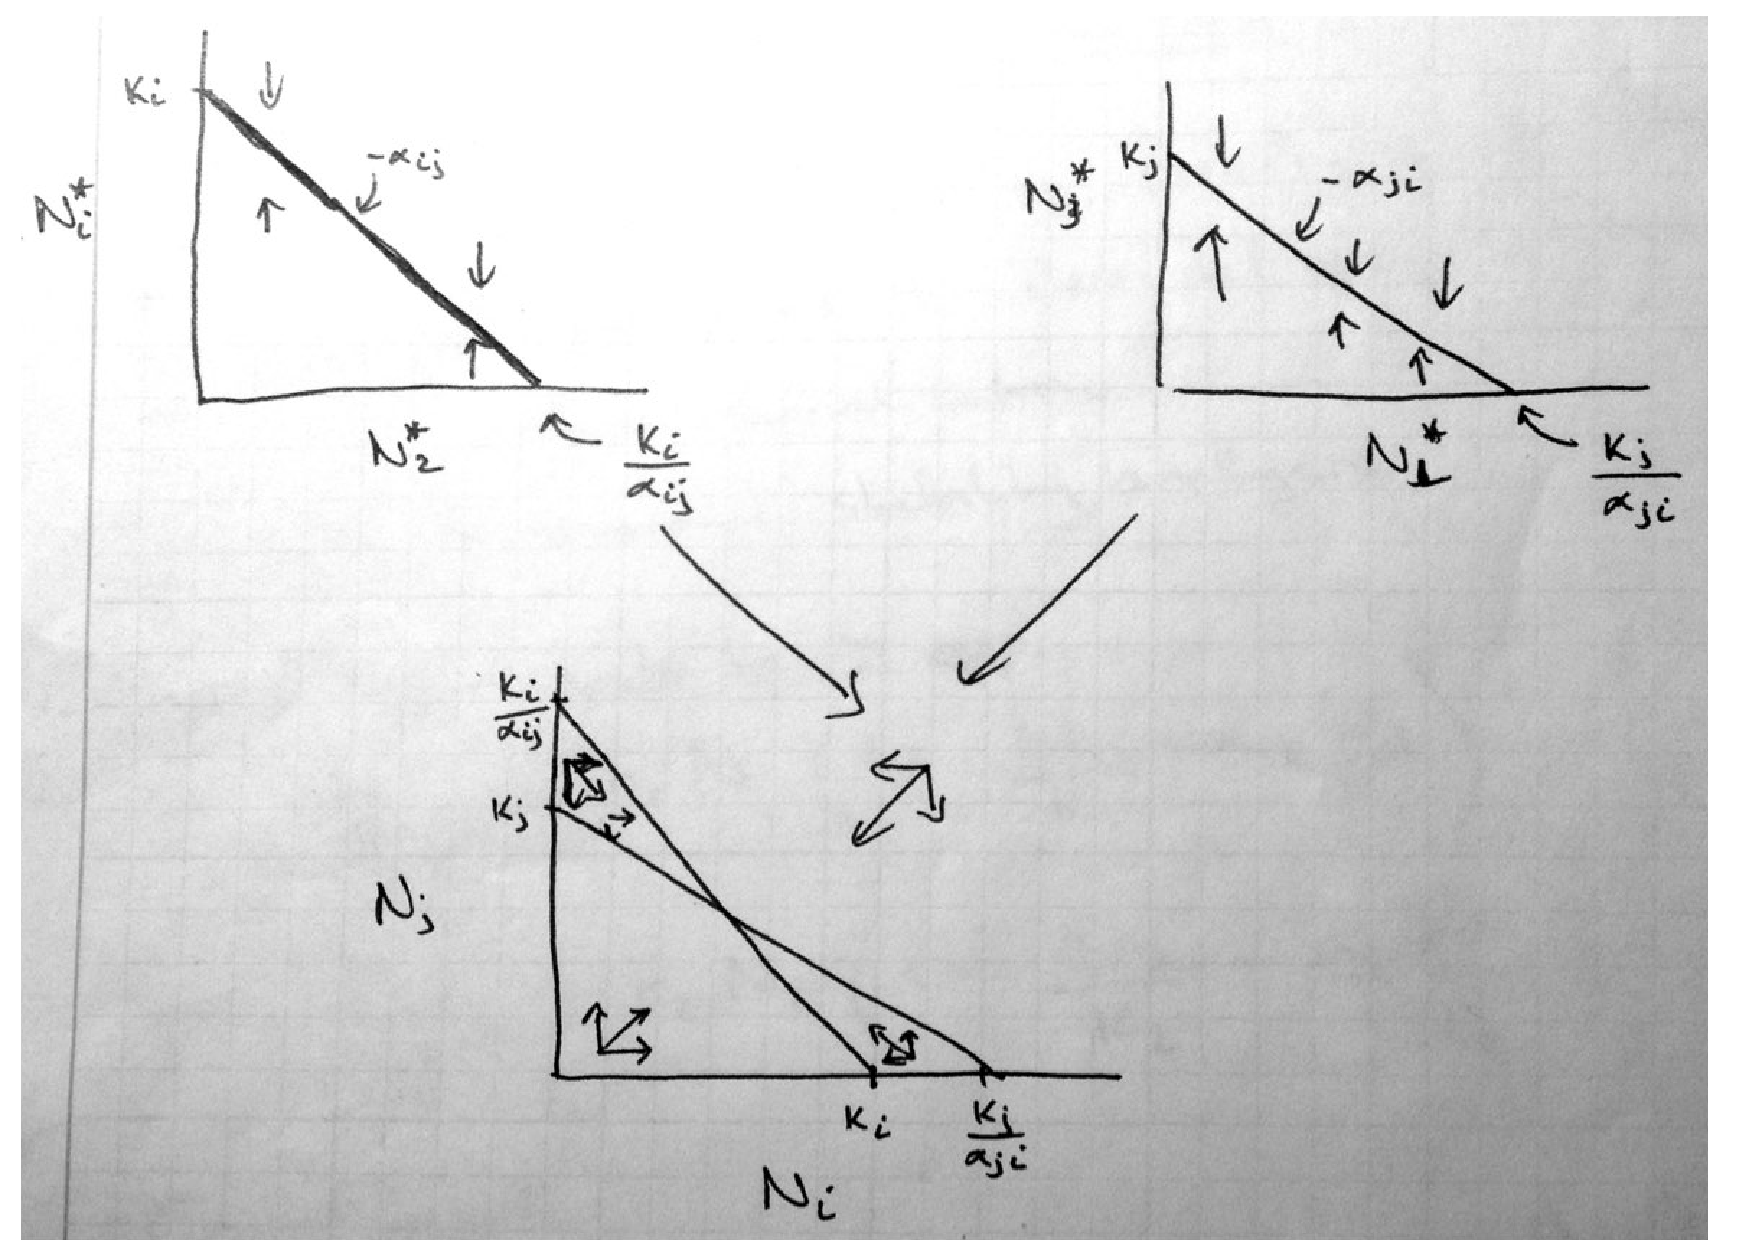
\includegraphics[width=17cm]{figs/LV_comp_isoclines.pdf}
\end{center}
\note{R-code: Work through other parameter values}\\

\textbf{Inferences/Conclusions:}

\begin{table*}[h]
\centering
\begin{tabular}{ll}
Coexistence: & intra $>$ inter for both species  \\
& \ind \ind (i.e. $\frac{K_i}{\alpha_{ii}}=\frac{K_i}{1} < \frac{K_j}{\alpha_{ji}} \Rightarrow \alpha_{ii}>\alpha_{ji}$)\\
Sp $i$ dominance: & intra $>$ inter for $i$ \& intra $<$ inter for $j$\\
Priority effect: & intra $<$ inter for both\\
& \ind \ind (i.e. $\frac{K_i}{\alpha_{ii}}=\frac{K_i}{1} > \frac{K_j}{\alpha_{ji}} \Rightarrow \alpha_{ii}<\alpha_{ji}$)
\end{tabular} 
\end{table*}

\rule[0.5ex]{\linewidth}{1pt}
\rule[0.5ex]{\linewidth}{1pt}


\end{document}